\documentclass[12pt,american]{report}
\usepackage{times}
\usepackage[T1]{fontenc}
\usepackage[utf8]{inputenc}
\usepackage{graphicx}
\usepackage{geometry}
\usepackage{siunitx}
\usepackage{pgfplots}
\usepackage{hyperref}
\usepackage{longtable}
\usepackage{caption}
\usepackage{url}
\usepackage{grffile}
\usepackage{ulem}
\usepackage{booktabs}
\usepackage{fancyvrb}
\usepackage{amssymb}
\usepackage{amsmath}
\usepackage{ifxetex}
\usepackage{ifluatex}
\geometry{verbose,letterpaper,tmargin=1in,bmargin=1in,lmargin=1.5in,rmargin=1in} %% sets paper size and margins
\usepackage{setspace}
\usepackage[square]{natbib}
\bibliographystyle{unsrtnat}
\usepackage{texments}
% \usepackage{amssymb}
\usepackage[]{algorithm2e}
\usestyle{xcode}


%\singlespacing        %% 1-spacing (default)
%\onehalfspacing       %% 1,5-spacing
%\doublespacing        %% 2-spacing

\pagestyle{plain}      %% select plain page style: no headers, page numbers center bottom

%% uncomment the following to include headers (e.g., to keep track of draft versions). Also change pagestyle to fancyplain:
%\rhead[\fancyplain{}{\leftmark}]%0
%      {\fancyplain{}{Draft 04/08 -- \thepage}}
%\cfoot[\fancyplain{Draft 04/08 -- \thepage}{}]{\fancyplain{Draft 04/08 -- \thepage}{}}

\begin{document}

\pagenumbering{roman}        %% roman page numbers for front matter

\renewcommand\thepage{}
\pagestyle{plain}
\begin{center}
\textbf{FOLDLINGS: an Interface for Interactive Pop-Up Card Design}
\vspace{0.4cm}

A Thesis\\ [0.4cm]
Submitted to the Faculty \\ [0.4cm]
in partial fulfillment of the requirements for the \\[0.4cm]
degree of \\[0.4cm]
Master of Science\\in\\Computer Science with a Concentration in Digital Arts\\[0.4cm]
by\\[0.5cm]
Nook Harquail\\[0.4cm]
in Conjunction with Marissa Allen \\[0.5cm]
Department of Computer Science \\ [0.4cm]
DARTMOUTH COLLEGE \\ [0.4cm]
Hanover, New Hampshire \\[0.4cm]
September 1, 2015 % that you will submit your signed thesis
\vspace{1.5cm}

\end{center}

Examining Committee:

\begin{flushright}
Advisor \line(180, 0){110} \\
Emily Whiting \\[1cm]

Member \line(180, 0){110} \\
Lorie Loeb \\[1cm]

Member \line(180, 0){110} \\
Jodie Mack \\[1cm]

% Member \line(180, 0){110} \\
% MEMBER NAME HERE\\[1cm]

%(ALL signatures must be in Black ink, ALL fonts in black ink)

\end{flushright}

\begin{flushleft}
\line(180, 0){110} \\
F. Jon Kull, Ph.D.\\
Dean of Graduate Studies\\[1cm]
%NOTE: the copies you submit must have the original signatures for PhD, one hard copy, for MS, two copies and a pdf of the thesis is required for both degrees.  No Holes, clips or binding on the copy and should be on Quality paper, preferably, Dartmouth Bond.
\end{flushleft}

% \pagestyle{plain}
\begin{center}
\textbf{FRAMESHIFT: SHIFT YOUR ATTENTION, SHIFT THE STORY}
\vspace{0.4cm}

A Thesis\\ [0.4cm]
Submitted to the Faculty \\ [0.4cm]
in partial fulfillment of the requirements for the \\[0.4cm]
degree of \\[0.4cm]
Master of Science\\in\\Computer Science with a Concentration in Digital Arts\\[0.4cm]
by\\[0.5cm]
Tim Tregubov\\[0.4cm]
in Conjunction with Rukmini Goswami \\[0.5cm]
Department of Computer Science \\ [0.4cm]
DARTMOUTH COLLEGE \\ [0.4cm]
Hanover, New Hampshire \\[0.4cm]
May 15, 2015 % that you will submit your signed thesis
\vspace{1.5cm}

\end{center}

Examining Committee:

\begin{flushright}
Chair \line(180, 0){110} \\
Lorie Loeb\\[1cm]

Member \line(180, 0){110} \\
Michael Cohen \\[1cm]

Member \line(180, 0){110} \\
Michael Casey \\[1cm]

% Member \line(180, 0){110} \\
% MEMBER NAME HERE\\[1cm]

%(ALL signatures must be in Black ink, ALL fonts in black ink)

\end{flushright}

\begin{flushleft}
\line(180, 0){110} \\
F. Jon Kull, Ph.D.\\
Dean of Graduate Studies\\[1cm]
%NOTE: the copies you submit must have the original signatures for PhD, one hard copy, for MS, two copies and a pdf of the thesis is required for both degrees.  No Holes, clips or binding on the copy and should be on Quality paper, preferably, Dartmouth Bond.
\end{flushleft}







% \include{TitlePage2}
\newpage
% a blank page follows the title page, this page is not numbered
\mbox{}
\newpage

\renewcommand\thepage{\arabic{page}}
\pagenumbering{roman}        %% roman page numbers for front matterstarting with page ii
\setcounter{page}{2}


% \renewcommand\thechapter{\arabic{chapter}.}
\renewcommand\thesection{\Roman{section}.}
\renewcommand\thesubsection{(\alph{subsection})}

\doublespacing               %% set spacing to double

\pagestyle{plain}
\begin{center}


\section*{ABSTRACT}


\end{center}
Crafting a 3D paper pop-up can be a lot of fun, and can help develop spatial reasoning skills.  However, designing the cuts and folds is often a frustrating trial and error process.  Foldlings is an iPad application that assists in this exploratory process.   Our tool-based approach allows users of all skill levels to create complex cards with ease, separating folding geometries into logical units.  This thesis focusses on the user interface and algorithms used in creating the two-dimensional view of the popup card from user input.

\cleardoublepage

\pagestyle{plain}
\begin{center}


\section*{Acknowledgements}

Thanks to Marissa Allen, my collaborator on this project, and co-author of chapters X and Y. \\
Special thanks Tim Tregubov, for working with us to develop the initial prototype for Foldlings, and for being a costant source of advice and technical help. \\
Thanks also to our advisors: Jodie Mack, Lorie Loeb, and Emily Whiting \\
Thanks to our first user: Rukmini Goswami.  Her feedback (and patience with our buggy software) were invaluable to us. \\
Thanks also to Kiko Lam and Luke Zirngibl for their feedback throughout the process.
\end{center}



\cleardoublepage


\singlespacing
\tableofcontents             %% include TOC
\listoftables                %% include list of tables
\listoffigures               %% include list of figures
\listofalgorithms        %% list of algos
\cleardoublepage             %% start new page

\pagenumbering{arabic}       %% arabic page numbers for body of text starting with page 1

\doublespacing
% \include{Introduction}

%START_INCLUDES

\chapter{Introduction}

\begin{figure}[htbp]
\centering
\includegraphics{figures/shared/01_Background/complexFoldlings.pdf}
\caption{A complex design created with our software.}
\end{figure}

\section{Background}\label{background}

\emph{This section is co-authored with Marissa Allen}

Kirigami is the art of papercraft originating from 17th century Japan
(\citet{temko1978magic}). Kirigami structures vary widely in form and
scale ---~from sub-microscopic creations to large sculptures
(\citet{grosso2015bending} to \citet{andrewscreating}). Kirigami can
represent a wide range of 2D and 3D constructions. For example, a design
can be a 2D lace-like pattern, or a large architectural structure; as
long as the paper design does not require glue or other attachments, it
is kirigami. Further constraints define subsets of kirigami --- such as
origami, which only allows folds\footnote{Purist origami adds further
  restrictions, including the requirement that the starting piece of
  paper be square (\citet{burczykul}).}. In particular, Foldlings is
concerned with 90-degree pop-up cards, which have the additional
constraint that orthogonal relationships exist between planes. We do not
use glue or other attachments in building pop-up cards; all designs are
cut from a single piece of paper, in the tradition of kirigami
(\citet{temko1978magic}). Thus, Foldlings creates orthogonal, kirigami
popup cards.

\begin{figure}[htbp]
\centering
\includegraphics{figures/shared/01_Background/popup-diagram.pdf}
\caption{Cross-section of a popup card. Figure modified from
https://en.wikipedia.org/ wiki/File:Popup-diagram.svg.}
\end{figure}

Typically, users create popup cards manually. For example, a user might
sketch out shape on a card in pencil, and then measure with a ruler to
determine where to place folds. Or, they might fold the paper while
cutting, discovering correct fold positions experimentally. The second
method works well for simple designs, but becomes difficult with complex
and nested geometries\footnote{These are behaviors we observed by
  watching users create pop-up cards.}. Constructing popup cards
manually is difficult for several reasons:

\begin{enumerate}
\def\labelenumi{\arabic{enumi}.}
\itemsep1pt\parskip0pt\parsep0pt
\item
  \textbf{2D to 3D visualization is difficult}. Users have difficulty
  understanding how the card will fold based on a 2D design.
\item
  \textbf{Geometric constraints}. Pop-up cards present strict
  constraints, which are often unintuitive to novice designers.
\item
  \textbf{No "undo"}. Since pop-up card design is often a
  trial-and-error process, designers must sometimes make multiple
  versions of their card to test their design.
\item
  \textbf{Physical constraints}. In addition to the geometric
  constraints, the paper medium presents physical limitations on where
  edges can be placed.
\end{enumerate}

The 90-degree popup card presents a tightly-constrained problem, with
opportunities for both interface design and algorithm innovations. Our
work spans human-computer interaction, graph-based algorithms, and
algorithms for manipulating bezier paths and pop-up card structures. Our
culminating product is an iPad application.

We present a system for designing popup cards, whose audience is
deliberately broad. That is, our tool aims to make the design process
easier and more fun for users with all degrees of popup card design
experience.

\section{Overview}\label{overview}

\emph{This section is co-authored with Marissa Allen}

\section{Related Work}\label{related-work}

\emph{This section is co-authored with Marissa Allen}

The only

\chapter{Design}

\section{Design Philosophy}\label{design-philosophy}

Our design philosophy is simple: follow the user. Following a
methodology roughly following agile methodologies, we . Development
driven rather than design driven.

mention affordances of iPad --- cite Gibson/teapot guy. We chose to
design for the iPad to

In practice, this has taken the form.

Throughout,

We strive to design an interface that is modular, friendly, and
delightful. Modularity stems from the decoupling of.

Friendliness is seen in the careful structuring of our experience to
make the design process . Delight comes from small details that . For
example, we

Construction paper

modularity friendliness delight

\section{Interface Iteration}\label{interface-iteration}

\begin{quote}
\begin{quote}
TODO: figure showing alpha UI
\end{quote}
\end{quote}

discuss move from drawing cuts \& folds directly to templating

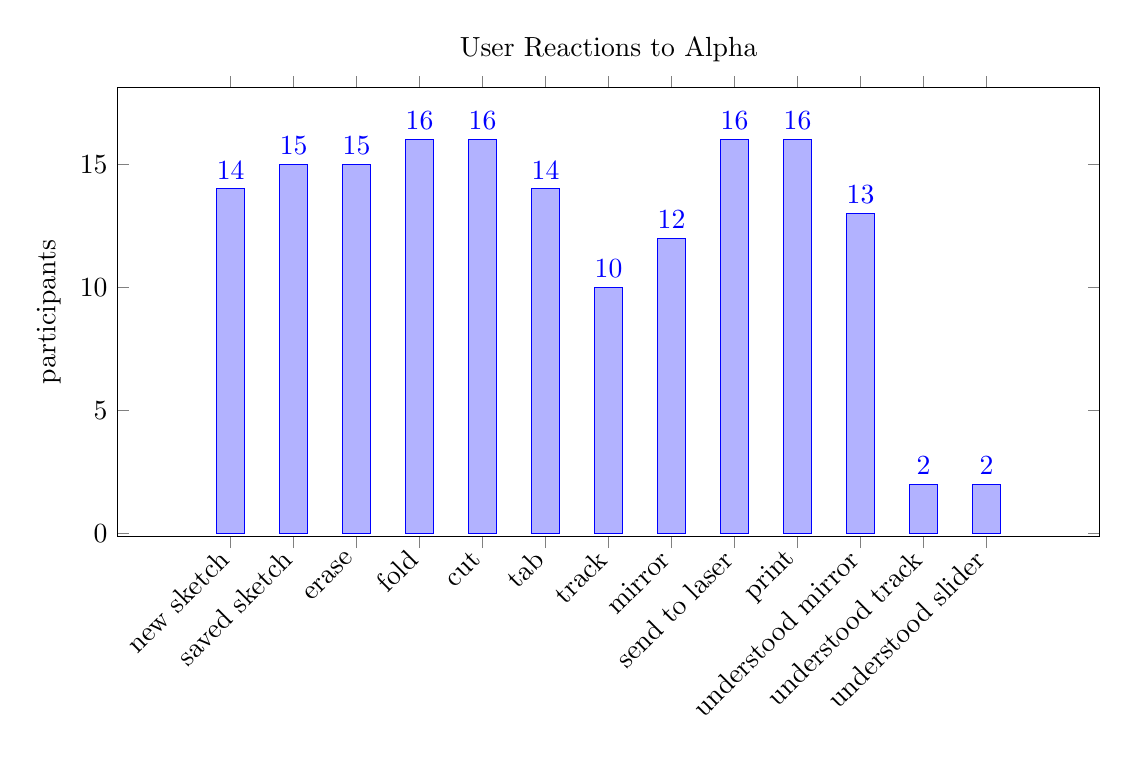
\begin{tikzpicture}
  \begin{axis}[
    title=User Reactions to Alpha,
    ybar,
    enlargelimits=0.15,
    x=0.8cm,
    legend style={at={(0.5,-0.2)},
      anchor=north,legend columns=-1},
    ylabel={participants},
    symbolic x coords={new sketch,saved sketch,erase,fold,cut,tab,track,mirror,send to laser,print,understood mirror,understood track,understood slider},
    xtick=data,
    nodes near coords, 
    nodes near coords align={vertical},
    x tick label style={rotate=45,anchor=east},
    ]
    \addplot coordinates {(new sketch,14)(saved sketch,15)(erase,15)(fold,16)(cut,16)(tab,14)(track,10)(mirror,12)(send to laser,16)(print,16)(understood mirror,13)(understood track,2)(understood slider,2)};
  \end{axis}
\end{tikzpicture}

\textbf{\textgreater{}\textgreater{}TODO: separate user comments from
observation}

\begin{longtable}[c]{@{}l@{}}
\caption{Feedback from first user test.}\tabularnewline
\toprule
\begin{minipage}[b]{0.82\columnwidth}\raggedright\strut
Comments
\strut\end{minipage}\tabularnewline
\midrule
\endfirsthead
\toprule
\begin{minipage}[b]{0.82\columnwidth}\raggedright\strut
Comments
\strut\end{minipage}\tabularnewline
\midrule
\endhead
\begin{minipage}[t]{0.82\columnwidth}\raggedright\strut
want option to fold other way, wanted to be able to draw over exising
line with tab tool, made a cake, crashed on returning to sketch
\strut\end{minipage}\tabularnewline
\begin{minipage}[t]{0.82\columnwidth}\raggedright\strut
track and slider will need explanation; wanted to use non-horizontal
folds
\strut\end{minipage}\tabularnewline
\begin{minipage}[t]{0.82\columnwidth}\raggedright\strut
wanted to fold by pinching, want to rename? delete, move them around?
\strut\end{minipage}\tabularnewline
\begin{minipage}[t]{0.82\columnwidth}\raggedright\strut
wanted ortho views, hold to view info about tool, examples. Interactive
tutorial
\strut\end{minipage}\tabularnewline
\begin{minipage}[t]{0.82\columnwidth}\raggedright\strut
erased master fold, crashing at preview step
\strut\end{minipage}\tabularnewline
\begin{minipage}[t]{0.82\columnwidth}\raggedright\strut
wanted interactive tutorials, made a cat
\strut\end{minipage}\tabularnewline
\begin{minipage}[t]{0.82\columnwidth}\raggedright\strut
momentary confusion getting back to sketch
\strut\end{minipage}\tabularnewline
\begin{minipage}[t]{0.82\columnwidth}\raggedright\strut
wanted to move around existing sketches
\strut\end{minipage}\tabularnewline
\begin{minipage}[t]{0.82\columnwidth}\raggedright\strut
confused about concept of a laser cutter
\strut\end{minipage}\tabularnewline
\begin{minipage}[t]{0.82\columnwidth}\raggedright\strut
wanted interative tutorial
\strut\end{minipage}\tabularnewline
\begin{minipage}[t]{0.82\columnwidth}\raggedright\strut
wanted to fold 3d preview by hand
\strut\end{minipage}\tabularnewline
\begin{minipage}[t]{0.82\columnwidth}\raggedright\strut
very frustrated by tools that aren't implemented yet
\strut\end{minipage}\tabularnewline
\begin{minipage}[t]{0.82\columnwidth}\raggedright\strut
confused by track \& slider
\strut\end{minipage}\tabularnewline
\begin{minipage}[t]{0.82\columnwidth}\raggedright\strut
needed heavy guidance; completely confused by track/slider
\strut\end{minipage}\tabularnewline
\begin{minipage}[t]{0.82\columnwidth}\raggedright\strut
wanted more snapping/guidance on creating valid designs
\strut\end{minipage}\tabularnewline
\begin{minipage}[t]{0.82\columnwidth}\raggedright\strut
fairly self-sufficient after tools were explained, made a house, moved
slowly, waiting for planes to calculate
\strut\end{minipage}\tabularnewline
\bottomrule
\end{longtable}

\section{Interactions}\label{interactions}

Through the iterations described in the previous chapter, we arrived at
Foldlings' tool-based system for card design.

\subsection{Tool Interactions}\label{tool-interactions}

Some interactions are common to all features. To add a feature . Tool
modes

\begin{quote}
\begin{quote}
TODO: add tap options, how to draw, and a description of the tool-based
interface in general
\end{quote}
\end{quote}

\subsubsection{Box Fold}\label{box-fold}

To draw a

\subsubsection{FreeForm}\label{freeform}

\subsubsection{Polygon}\label{polygon}

\subsubsection{V-Fold}\label{v-fold}

The only action that can be performed on a v-fold feature is deletion.

\subsection{Tutorial}\label{tutorial}

We eschewed detailed drawing instructions or a separate tutorial mode,
in favor of short video tutorials that appear the first time each tool
is used. These tutorials can also be accessed by tapping the feature
icons on the about page.

\begin{figure}[htbp]
\centering
\includegraphics{figures/32_UI_Tool_Interactions/tutorial_step_one_two.png}
\caption{Free-form shape tutorial video.}
\end{figure}

We also show helpful tips between screens --- for example, when moving
to 3D preview and restoring from a saved sketch.

\subsection{Warnings and Errors}\label{warnings-and-errors}

We display warnings and errors as bright-red banners at the top of the
sketch view when. These warnings are displayed in response to failing
the validity checks performed when adding a feature to the sketch.

\begin{figure}[htbp]
\centering
\includegraphics{figures/32_UI_Tool_Interactions/error_message.png}
\caption{An error message shown when rejecting a polygon with
intersecting edges.}
\end{figure}

The goal of these warnings is to give users descriptive feedback when
errors occur, and to give them an intuitive sense of which actions
create invalid features.

\subsection{Send to Laser Cutter}\label{send-to-laser-cutter}

In the three-dimensional preview, users can tap the ``send to laser
cutter'' option. This feature sends the user an email with an attached
SVG file. This file can be fed to a laser cutter or paper cutting
machine, or can be opened in a vector graphics program to make further
changes.

\subsection{Print}\label{print}

\begin{figure}[htbp]
\centering
\includegraphics{figures/32_UI_Tool_Interactions/tutorial_step_one_two.png}
\caption{Options for sharing a fold pattern from the 3D preview.}
\end{figure}

\section{Interface Data Structures}\label{interface-data-structures}

We will refer to several data structures throughout the discussion of
user interface design and implementation. These are the primary means of
storing user input processed by the tools, and are processed by our
algorithms to draw designs in 2D and simulate them 3D\footnote{This
  section only describes the primary data structures necessary for
  constructing fold and patterns from user input, detecting planes, and
  determining the relationships between, not the systems for drawing
  features in 2D or 3D. For a discussion of 2D drawing, see sections.
  For a discussion of, see .
  \textbf{\textgreater{}\textgreater{}TODO:cite marissa
  \textgreater{}\textgreater{}TODO reference section}}.

\subsection{Edges}\label{edges}

An Edge represents a cut or fold. Edges are the basic building block of
planes, and an integral element of all fold features. An edge is
minimally defined by a start point, end point, and a a type (either cut
or fold). This minimal definition represents a straight edge between two
points. In addition, an Edge can contain further information: the bezier
path drawn to create it (for non-straight edges), and a reference to the
plane or feature it is a part of. Additionally, each edge contains a
reference to its ``twin'' edge.

\subsubsection{Twin Edges}\label{twin-edges}

Although it is often simplest to think of edges as cuts and folds
created by the user, the reality in Foldlings is slightly more
complicated. For each edge that the user creates using a tool, two edges
are created. We create edges with direction, such that there is an edge
from the start point to the end point of the edge, and another edge
starts at the endpoint and has the reverse path of the original edge.
This distinction is most important when detecting planes from
edges\footnote{\textbf{\textgreater{}\textgreater{}TODO cite marissa's
  planes}}, but must also be taken into account whenever edges are
processed. For example, when drawing the 2D view of a sketch, we skip
drawing the twins of edges already drawn, which reduces drawing work by
half.

\begin{figure}[htbp]
\centering
\includegraphics{figures/33_UI_Interface_Data_Structures/boxfold_34_edges.png}
\caption{This sketch contains 34 edges, with orientations shown by the
overlaid gray arrows.}
\end{figure}

\subsubsection{Driving Folds}\label{driving-folds}

A driving fold is not a special type of edge, but rather a relationship
between an edge in one feature and a feature ``spanning'' that edge. A
feature is said to span a fold when it is drawn on top of an existing
fold, so that it has horizontal folds on both sides of the middle fold.

\begin{figure}[htbp]
\centering
\includegraphics{figures/33_UI_Interface_Data_Structures/boxfold_driving_non_driving.png}
\caption{Left: a box fold mid-drag. The feature does not have a driving
fold. Right: a box-fold after the user has released the touch. The
feature's driving fold is the master card's middle horizontal fold.}
\end{figure}

An edge can be the driving fold for more than one feature, but each
feature has only one driving fold (if there are multiple potential
driving edges at the same height, the leftmost edge is selected. The
driving fold is important for calculating parent-child relationships
between features: a feature's parent is the feature that contains it's
driving fold\footnote{The exception to this rule is holes ---~a hole's
  parent is the feature that contains it.}. These parent-child
relationships are described in more detail in the
\nameref{nested-features} section on page \pageref{nested-features}.

\subsubsection{Fold Orientation}\label{fold-orientation}

Traditionally, kirigami patterns are based on.
\textbf{\textgreater{}\textgreater{}TODO: FINISH SECTION, cite}
\textbf{\textgreater{}\textgreater{} TODO KIRIGAMI PATTERN FIGURE}

\subsection{Planes}\label{planes}

Planes are an enclosed shape, bounded by edges. Plane are detected from
edges by traversing the directed edge graph, as describe in
\textbf{\textgreater{}\textgreater{}TODO: CITE MARISSA HERE}. They are
drawn as colored areas in the two-dimensional sketch, and simulated in
the 3D preview as shapes that rotate about a pivot point. In order to
simulate the planes in 3D, we construct parent-child relationships
between the planes, which determine how they move during simulation.

\begin{figure}[htbp]
\centering
\includegraphics{figures/33_UI_Interface_Data_Structures/boxfold_planes.png}
\caption{Planes in a simple sketch, numbered by ancestry. Starting at
the root plane 1, each successive plane is the child of the previous
numbered plane.}
\end{figure}

\subsection{Fold Features}\label{fold-features}

The central data structure of Foldlings is the FoldFeature: a
representation of a shape drawn by the user that folds in 3d. Each fold
feature is a single design element ---~and can be individually created,
modified, and deleted. There are five classes of FoldFeature:
MasterCard, BoxFold, FreeForm, Polygon, and V-Fold, representing
differences in drawing behavior, geometry, and (the differences are
described in detail below). Each of these features is a subclass of the
FoldFeature superclass.

All FoldFeatures have functionality in common:

\begin{itemize}
\itemsep1pt\parskip0pt\parsep0pt
\item
  Each feature contains a list of edges in the feature ---~cuts and
  folds, including twins.
\item
  Each feature has a driving fold --- in the case of unconnected
  features, such as the master card and holes, the driving fold is nil.
\item
  Each feature can be deleted from the Sketch, ``healing'' the sketch by
  closing gaps left in any
\item
  Features implement the encodeWithCoder and decodeWithCoder methods,
  allowing them to be serialized to a file on the device and restored
  from the saved file.
\item
  Each feature can provide a list of current ``tap options'' --- actions
  that can be performed on the feature given its state.
  \textbf{\textgreater{}\textgreater{}TODO:SEE tap options in interface
  design}
\item
  Each feature can perform hit-testing: given a point, it can determine
  whether that point is inside or outside the feature. \citep{Nobody06}.
  \textbf{\textgreater{}\textgreater{}TODO:REMOVE CITATION -- JUST
  TESTING}
\end{itemize}

\subsubsection{Master Card}\label{master-card}

Each sketch always contains a single master feature, which is the
ancestor of all other features. It is a simplification of the box fold,
in that it contains three horizontal folds with connecting vertical
cuts. Users do not create features of this type~--- each sketch begins
with one. All of the edges in the master feature are marked with a flag
indicating that they belong to the master feature, because master
feature edges and planes are sometimes treated differently than normal
edges. For example, the parent-child relationships between planes are
constructed by starting at the top plane in the master feature,
determined by edge type and height.

\subsubsection{Box Fold}\label{box-fold}

A box fold consists entirely of straight edges, and can be constructed
from two points: the top left point, and the bottom right. The middle
fold position is determined by the position of the driving fold. Box
folds are only valid if they have a driving fold.

\subsubsection{Free Form}\label{free-form}

Free-form shapes are defined by a single, closed path. When the feature
is completed (by releasing the touch), the shape is truncated,
horizontal folds are added, and the path is split into multiple edges
(assuming the shape spanned a fold)\footnote{\textbf{\textgreater{}\textgreater{}TODO:SEE
  SECTION}}. The curved path is defined by a set of ``interpolation
points'' ---~points captured by sampling touch positions while a user
draws a shape on the screen. A bezier path is interpolated between these
points using the Catmull-Romm algorithm \textbf{TODO: CITE}.

Holes are a special case of FreeForm shapes, and are cut out from the
final design, rather than folded. FreeForm shapes that do not cross a
fold are considered holes ---~drawn in white in the 2d sketch and drawn
as subtractions from planes in the 3d view.

\subsubsection{Polygon}\label{polygon}

Polygons are created from a list of ``tap points'' constructed from user
input. As in free-form shapes, these points are connected with a bezier
path, and are truncated if they contain a driving fold when they are
completed. For polygons, this path consists only of straight line
segments. Unlike interpolation points, tap points can be moved at any
time during the drawing process.

Like FreeForm shapes, Polygons that do not have a driving fold are
considered holes.

\subsubsection{V-Fold}\label{v-fold}

V-Folds are defined by a path that crosses the driving fold, called a
``vertical cut.'' This path can be an arbitrary shape that crosses the
driving fold once. They are fully-defined by adding a point on the
driving fold. From this point, we construct three diagonal folds, two to
the top and bottom of the vertical cut, and one to a point that
intersects with the vertical cut at a point calculated to make a valid
90-degree feature.

\begin{figure}[htbp]
\centering
\includegraphics{figures/33_UI_Interface_Data_Structures/vfold_before_after.png}
\caption{Left: the vertical cut of a v-fold. Right: a v-fold after
defining the point on the driving fold to create diagonal cuts.}
\end{figure}

V-folds are only valid if they have a driving fold, and their vertical
cut intersects the driving fold exactly once.

\subsection{Sketches}\label{sketches}

A sketch is the representation of the user's drawing ---~its primary
role is as a collection of features. It also contains information about
the current drawing state, and the state of user interaction (for
example, which features are currently being modified, and which tool is
selected).

\section{Saving}\label{saving}

afsdfs dsf sf

\chapter{Technical Contributions}

\section{Interface Implementation}\label{interface-implementation}

\textbf{\textgreater{}\textgreater{}TODO DIAGRAM OF SKETCH VIEW
CONTROLLER SKETCHVIEW CONTAINS SKETCH CONTAINS FEATURES}

description of drawing, touch handling, etc. catmull rom curves showing
feature state

Cite model v (\citet{veit2003model}).

\subsection{Touch Handling}\label{touch-handling}

In order to create features, the first step. In almost all cases,

\section{Tool Implementation}\label{tool-implementation}

Below is the definition of the FoldFeature superclass --- all features
created using Foldlings can override these methods to provide specific
functionality. For further discussion of the FoldFeature data structure,
see \textbf{\textgreater{}\textgreater{}TODO cite}.

\singlespacing 

\begin{pygmented}{swift}
var horizontalFolds:[Edge] = [] //list of horizontal folds
var featureEdges:[Edge]?        //edges in a feature
var children:[FoldFeature] = [] // children of feature
var drivingFold:Edge? // driving fold of feature
var parent:FoldFeature? // parent of feature
var startPoint:CGPoint?
var endPoint:CGPoint? // start and end touch points

/// splits an edge around the current feature
func splitFoldByOcclusion(edge:Edge) -> [Edge]
{
//by default, return edge whole
return [edge]
}
/// features are leaves if they don't have children
func isLeaf() -> Bool
{
return children.count == 0
}
/// options or modifications that can be made to the current feature
func tapOptions() -> [FeatureOption]?
{
  return [FeatureOption.PrintPlanes, FeatureOption.PrintEdges,
  FeatureOption.ColorPlaneEdges, FeatureOption.PrintSinglePlane]
}
/// whether a feature is drawn over a fold, determines whether 
/// a fold can be the driving fold for a feature
  func featureSpansFold(fold:Edge)->Bool
{
  return false
}
/// returns and calculates planes in a feature
func getFeaturePlanes()-> [Plane]{
  return featurePlanes
}
/// whether a feature contains a point
/// needs to be overridden by subclasses
func containsPoint(point:CGPoint) -> Bool{
  return self.boundingBox()?.contains(point) ?? false
}
\end{pygmented}

\doublespacing

\subsection{Box Fold}\label{box-fold}

talk about fold heights talk about occlusion

\subsubsection{FreeForm}\label{freeform}

talk about truncation talk about splitting

\begin{algorithm}[H]
 \KwData{this text}
 \KwResult{how to write algorithm with \LaTeX2e }
 initialization\;
 \While{not at end of this document}{
  read current\;
  \eIf{understand}{
   go to next section\;
   current section becomes this one\;
   }{
   go back to the beginning of current section\;
  }
 }
 \caption{Path Splitting}
\end{algorithm}

\subsubsection{Polygon}\label{polygon}

contrast with free-form talk about point dragging talk about truncation

\subsubsection{V-Fold}\label{v-fold}

talk about angle calculation

\section{Intersections Between
Features}\label{intersections-between-features}

As we observed at the Digital Arts Exhibition \footnote{see}, users
often attempt to draw features that overlap with existing features in
the sketch. This is a difficult, and is only partly implemented due to
the complexity involved in adding intersections to our system.

\textbf{\textgreater{}\textgreater{}TODO algorithm}

\section{Feature Validity}\label{feature-validity}

Each feature contains a

\section{Constraints on Fold
Features}\label{constraints-on-fold-features}

\subsection{Geometric Constraints}\label{geometric-constraints}

\subsubsection{Box Fold}\label{box-fold}

\subsubsection{Freeform}\label{freeform}

\subsubsection{Polygon}\label{polygon}

\subsubsection{V-Fold}\label{v-fold}

\subsection{Physical Constraints}\label{physical-constraints}

Physical. Obvious . Minimum edge length. This depends on the laser
cutter

\textbf{\textgreater{}\textgreater{}TODO: Figure showing problem}

\include{chapters/50_User_Study_Dax}
\section{Visual Aids User Study}\label{visual-aids-user-study}

\begin{figure}[htbp]
\centering
\includegraphics{figures/51_User_Study_Visual_Aids/kikofoldling.jpg}
\caption{A Participant folding a card in our study on 2D to 3D visual
aids for popup cards.}
\end{figure}

The goal of this study was to determine whether users understand the
mapping of 2d fold patterns to 3D, and test the degree to which plane
shading, edge patterning, and a 3D preview help users understand how a
popup card will fold.

\textbf{\textgreater{}\textgreater{}TODO: cite other research on visual
aids for folding slash other 2d to 3D vis}

\subsection{Method}\label{method}

We performed this study with 22 participants, who spent an average of 18
minutes with us. Each subject received a set of five laser cut cards,
and we recorded the time for them to successfully fold the card.
Although there was some variety in age and background, but the largest
demographic was undergraduate Dartmouth students. 10 of the participants
were male, 12 were female.

For each card, each subject was randomly given one of of the following
five aids:

\begin{enumerate}
\def\labelenumi{\arabic{enumi})}
\itemsep1pt\parskip0pt\parsep0pt
\item
  A two-dimensional design, showing planes shaded by whether they will
  be horizontal or vertical when folded.
\item
  A two-dimensional design, with edges patterned based on whether they
  are ``hills'' or ``valleys'' --- whether they fold towards or away
  from the card.
\item
  A video showing a simulation of the card folding in three dimensions.
\item
  A still image of the card folded in dimension.
\item
  No visual aid.
\end{enumerate}

The order of aids and cards was shuffled, and then balanced to ensure an
equal distribution of orderings. I.e each visual aid has an equal chance
of being the first aid presented to a user and the last aid presented.

Finally, we asked subjects to rank the visual aids in order of most to
least helpful. For materials used in the study, see Appendix A.

\subsection{Results and Discussion}\label{results-and-discussion}

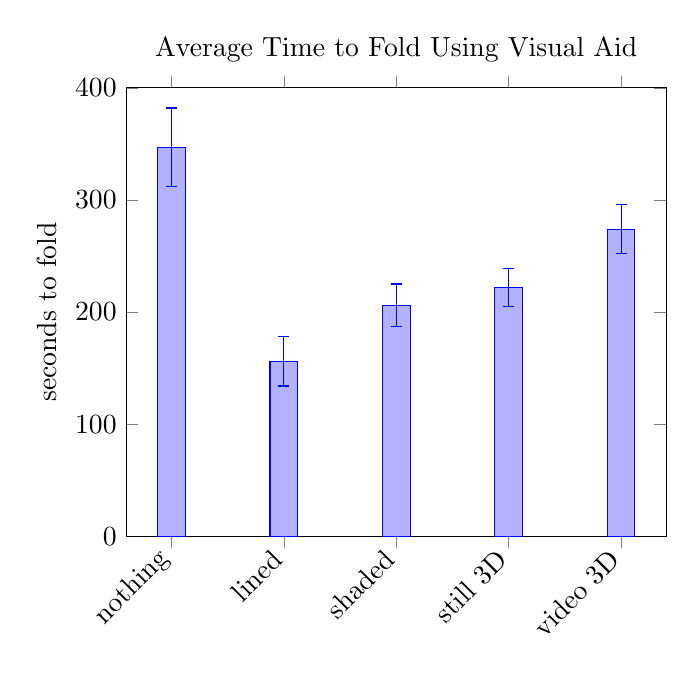
\begin{tikzpicture}
\begin{axis}[
  title=Average Time to Fold Using Visual Aid,
    ybar,
    ymin=0, ymax=400,
    legend style={at={(0.5,-0.2)},
     legend columns=-1},
    ylabel={seconds to fold},
    symbolic x coords={nothing,lined,shaded,still 3D,video 3D},
    xtick=data,
    x tick label style={rotate=45,anchor=east},
]
\addplot+[error bars/.cd,
y dir=both,y explicit]
coordinates {
    (nothing,347) +- (0.0, 35)
    (lined,156) +- (0.0, 22)
    (shaded,206) +- (0.0, 19)
    (still 3D,222) +- (0.0, 17)
    (video 3D,274) +- (0.0, 22)};
\end{axis}
\end{tikzpicture}

The time to fold varied significantly depending on the visual aid used
to fold the card. Error bars indicate a 95\% confidence interval around
the mean, showing a relatively narrow variance within each visual aid
data set. From this, we can conclude that trials with no visual aid were
slower than all trails with visual aids, and that the lined pattern
showing fold orientation was more helpful that any other preview method.
While the shaded visual aid and still 3D preview were indistinguishable,
video 3D was slightly worse than all other visual aids.

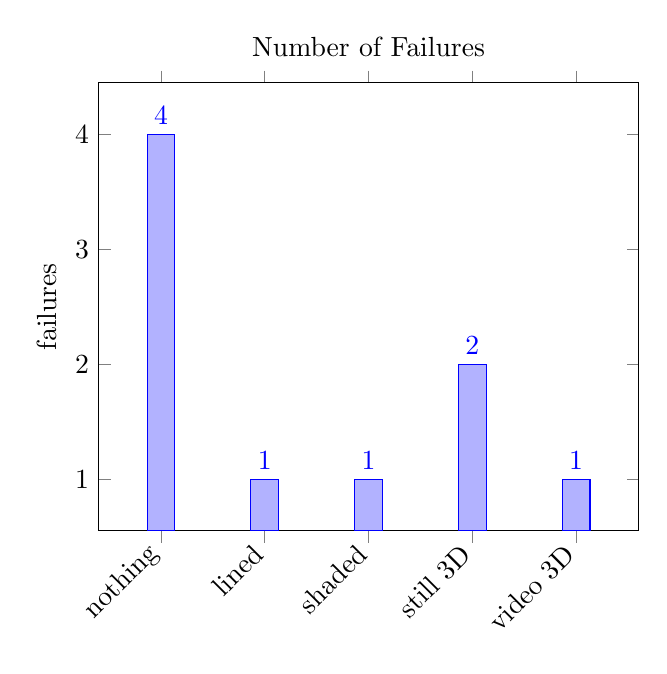
\begin{tikzpicture}
  \begin{axis}[
    title=Number of Failures,
    ybar,
    enlargelimits=0.15,
    legend style={at={(0.5,-0.2)},
      anchor=north,legend columns=-1},
    ylabel={failures},
    symbolic x coords={nothing,lined,shaded,still 3D,video 3D},
    xtick=data,
    nodes near coords, 
    nodes near coords align={vertical},
    x tick label style={rotate=45,anchor=east},
    ]
    \addplot coordinates {(nothing,4)(lined,1)(shaded,1)(still 3D,2)(video 3D,1)};
  \end{axis}
\end{tikzpicture}

Some trials were not completed successfully. In some cases, users folded
the design incorrectly --- in others, they refused to fold the card,
feeling lost without a visual aid. Unsurprisingly, users were far more
likely to fail to fold the card when they did not have a visual aid. The
times for these failures were not recorded in the Number of Figures
graph above.

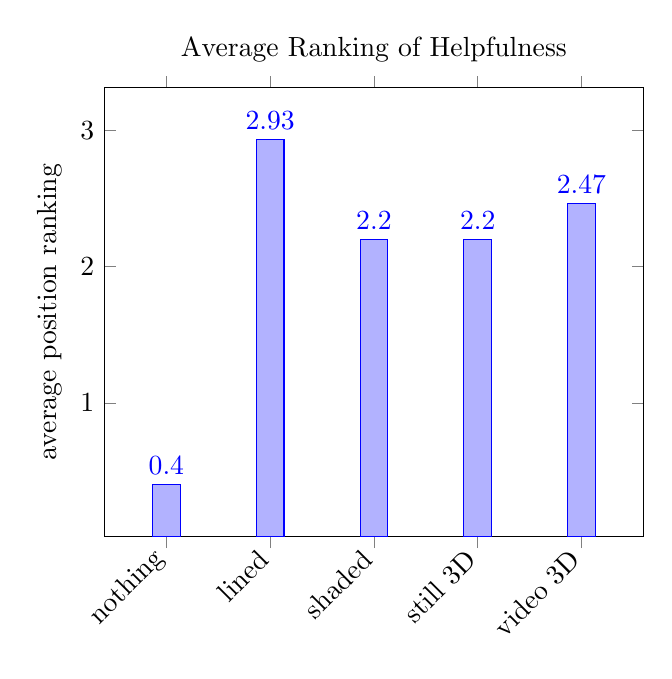
\begin{tikzpicture}
  \begin{axis}[
    title=Average Ranking of Helpfulness,
    ybar,
    enlargelimits=0.15,
    legend style={at={(0.5,-0.2)},
      anchor=north,legend columns=-1},
    ylabel={average position ranking},
    symbolic x coords={nothing,lined,shaded,still 3D,video 3D},
    xtick=data,
    nodes near coords, 
    nodes near coords align={vertical},
    x tick label style={rotate=45,anchor=east},
    ]
    \addplot coordinates {(nothing,0.4)(lined,2.933333333)(shaded,2.2)(still 3D,2.2)(video 3D,2.466666667)};
  \end{axis}
\end{tikzpicture}

We asked subjects to rank the visual aids from most to least helpful. In
this graph, the data is averaged and inverted (5 being the most
helpful), to show the relatively helpfulness of each aid. Participants
rated the lined aid as the most helpful~---~with small differences among
the other aids. The lack of visual aid rated very poorly.

While this study gives persuasive evidence for the relative helpfulness
of lines showing fold orientation, it is possible that other aids are
more helpful in completing other 2D to 3D visualization tasks. For
example, it would be interesting to compare the results if we asked
users to simply label horizontal and vertical planes instead of folding
a card. Perhaps the lined visual aid was most valuable to this task
because it was closest to the action participants performed: fold
orientation is very closely related to the task of folding a card.

Another limitation of this study is that we do not fully test the
effectiveness of our interactive 3D preview in helping users visualize
the folded card. We chose to limit the 3D video aid to a non-interactive
aid, to make it more directly comparable to the other visual
aids\footnote{If we allowed users to interact with the aid, they would
  have been physically split between interacting with the card and
  interacting with the 3D preview. Also, differences in familiarity with
  iPad use might have been a confounding factor if we had used a tablet
  to display the 3D preview.}. However, a key benefit of the 3D preview
in our software is that users can directly manipulate and rotate the
simulated card, which was not possible in this study.

In Foldlings, we implement many of these visual aids. In the 2D sketch,
we shade planes based on orientation, and display a 3D preview that
users can manipulate in the 3D preview. As a result of our findings in
this study, we also implemented line patterning based on fold
orientation for the SVG export.

\section{Final User Study}\label{final-user-study}

As a final test of software, we compared the usability with Foldlings to
traditional manual popup design methods. First, we presented
participants with a completed popup card, and asked them to replicate
the design using manual cutting and folding and to create the design
using our software. The order was randomized, so half of participants
were given were given the manual first, and half started with Foldlings.
We timed how long the participants took to complete the design. Next, we
gave them a free-form exercise: make a design that includes a tree."
Finally, we asked participants to rate the experience of using our tool
and their satisfaction with the popup card they produced.
\textgreater{}\textgreater{}TODO: attach image
\textgreater{}\textgreater{}TODO graphs, data, participants, do the
study lol

\textbf{\textgreater{}\textgreater{}TODO: update}

\chapter{Conclusions}

Foldlings. Plan to release Foldlings in the Apple app store. In many
ways, the

\section{User Interface Future Work}\label{user-interface-future-work}

\subsection{Multiple Cards}\label{multiple-cards}

\citet{hart2007modular}

\subsection{Horizontal}\label{horizontal}

\section{Algorithms \& Implementation Future
Work}\label{algorithms-implementation-future-work}

\subsection{Feature Intersections}\label{feature-intersections}

\subsection{Concurrency}\label{concurrency}

\section{Applications}\label{applications}

\emph{This section is co-authored with Marissa Allen}

\chapter{Appendix}

\captionsetup[figure]{list=no}

\section{Appendix A: User Interface
Mockups}\label{appendix-a-user-interface-mockups}

Mockups

\section{Appendix B: Designs Created at
DAX}\label{appendix-b-designs-created-at-dax}

Mockups

\section{Appendix C: Visual Aids User Study
Materials}\label{appendix-c-visual-aids-user-study-materials}

\subsection{Lined Visual Aids}\label{lined-visual-aids}

Lined cards indicating fold orientation ---~bold for hills, normal
emphasis for valleys.

\begin{figure}[htbp]
\centering

\includegraphics{figures/92_Appendix_Visual_Aids_Materials/lined_card1.png}
\caption{}
\end{figure}

\begin{figure}[htbp]
\centering
\includegraphics{figures/92_Appendix_Visual_Aids_Materials/lined_card2.png}
\caption{}
\end{figure}

\clearpage

\begin{figure}[htbp]
\centering

\includegraphics{figures/92_Appendix_Visual_Aids_Materials/lined_card3.png}
\caption{}
\end{figure}

\begin{figure}[htbp]
\centering

\includegraphics{figures/92_Appendix_Visual_Aids_Materials/lined_card4.png}
\caption{}
\end{figure}

\begin{figure}[htbp]
\centering

\includegraphics{figures/92_Appendix_Visual_Aids_Materials/lined_card5.png}
\caption{}
\end{figure}

\clearpage

\subsection{Shaded Visual Aids}\label{shaded-visual-aids}

Shaded cards indicating plane orientation ---~gray for horizontal, white
for vertical planes.

\begin{figure}[htbp]
\centering
\includegraphics{figures/92_Appendix_Visual_Aids_Materials/shaded_card1.png}
\caption{}
\end{figure}

\begin{figure}[htbp]
\centering
\includegraphics{figures/92_Appendix_Visual_Aids_Materials/shaded_card2.png}
\caption{}
\end{figure}

\clearpage

\begin{figure}[htbp]
\centering
\includegraphics{figures/92_Appendix_Visual_Aids_Materials/shaded_card3.png}
\caption{}
\end{figure}

\begin{figure}[htbp]
\centering
\includegraphics{figures/92_Appendix_Visual_Aids_Materials/shaded_card4.png}
\caption{}
\end{figure}

\begin{figure}[htbp]
\centering
\includegraphics{figures/92_Appendix_Visual_Aids_Materials/shaded_card5.png}
\caption{}
\end{figure}

\clearpage

\subsection{Still 3D Visual Aids}\label{still-3d-visual-aids}

Still 3d previews of the folded card.

\begin{figure}[htbp]
\centering
\includegraphics{figures/92_Appendix_Visual_Aids_Materials/still_card1.png}
\caption{}
\end{figure}

\begin{figure}[htbp]
\centering
\includegraphics{figures/92_Appendix_Visual_Aids_Materials/still_card2.png}
\caption{}
\end{figure}

\begin{figure}[htbp]
\centering
\includegraphics{figures/92_Appendix_Visual_Aids_Materials/still_card3.png}
\caption{}
\end{figure}

\begin{figure}[htbp]
\centering
\includegraphics{figures/92_Appendix_Visual_Aids_Materials/still_card4.png}
\caption{}
\end{figure}

\begin{figure}[htbp]
\centering
\includegraphics{figures/92_Appendix_Visual_Aids_Materials/still_card5.png}
\caption{}
\end{figure}

\clearpage

\subsection{Video Visual Aids}\label{video-visual-aids}

Note: these were displayed on a laptop screen as a video; only
screenshots are shown here.

\begin{figure}[htbp]
\centering
\includegraphics{figures/92_Appendix_Visual_Aids_Materials/video_card1.png}
\caption{}
\end{figure}

\begin{figure}[htbp]
\centering
\includegraphics{figures/92_Appendix_Visual_Aids_Materials/video_card2.png}
\caption{}
\end{figure}

\begin{figure}[htbp]
\centering
\includegraphics{figures/92_Appendix_Visual_Aids_Materials/video_card3.png}
\caption{}
\end{figure}

\begin{figure}[htbp]
\centering
\includegraphics{figures/92_Appendix_Visual_Aids_Materials/video_card4.png}
\caption{}
\end{figure}

\begin{figure}[htbp]
\centering
\includegraphics{figures/92_Appendix_Visual_Aids_Materials/video_card5.png}
\caption{}
\end{figure}

\clearpage

\subsection{Completed Cards}\label{completed-cards}

Cards folded by participants in the study.

\begin{figure}[htbp]
\centering
\includegraphics{figures/92_Appendix_Visual_Aids_Materials/completed_card1.png}
\caption{}
\end{figure}

\begin{figure}[htbp]
\centering
\includegraphics{figures/92_Appendix_Visual_Aids_Materials/completed_card2.png}
\caption{}
\end{figure}

\begin{figure}[htbp]
\centering
\includegraphics{figures/92_Appendix_Visual_Aids_Materials/completed_card3.png}
\caption{}
\end{figure}

\begin{figure}[htbp]
\centering
\includegraphics{figures/92_Appendix_Visual_Aids_Materials/completed_card4.png}
\caption{}
\end{figure}

\begin{figure}[htbp]
\centering
\includegraphics{figures/92_Appendix_Visual_Aids_Materials/completed_card5.png}
\caption{}
\end{figure}

\clearpage

\section{Appendix D: Separation of
Work}\label{appendix-d-separation-of-work}

This project is a collaboration between Marissa Allen and Nook Harquail.
Although we worked collaboratively on the software, each of us presents
an individual thesis paper. Our responsibilities on the software were as
follows: Nook concentrated on tools and interactions, including
performing user studies and processing user input, while Marissa
concentrated on implementing the 3D simulation and data structures,
including methods to define and render planes in 2D and 3D.

%END_INCLUDES

% \appendix
% 

\section*{Appendix A: User Study 1}
\addcontentsline{toc}{section}{Appendix A: User Study 1}

% \begin{figure}[h!]
% \begin{center}$
% \begin{array}{c c}
% \includegraphics[width=2.3in]{figures/exp1/test-01.png} &
% \includegraphics[width=2.3in]{figures/exp1/test-02.png} \\ 
% \includegraphics[width=2.3in]{figures/exp1/test-03.png} &
% \includegraphics[width=2.3in]{figures/exp1/test-04.png} \\ 
% \includegraphics[width=2.3in]{figures/exp1/test-05.png} &
% \includegraphics[width=2.3in]{figures/exp1/test-06.png} \\ 
% \includegraphics[width=2.3in]{figures/exp1/test-07.png} &
% \includegraphics[width=2.3in]{figures/exp1/test-08.png} \\ 
% \includegraphics[width=2.3in]{figures/exp1/test-09.png} &
% \includegraphics[width=2.3in]{figures/exp1/test-10.png}
% \end{array}$
% \end{center}
% \end{figure}

% \begin{figure}[h]
% \begin{center}$
% \begin{array}{c c}
% \includegraphics[width=2.5in]{figures/exp1/test-11.png} &
% \includegraphics[width=2.5in]{figures/exp1/test-12.png} \\ 
% \includegraphics[width=2.5in]{figures/exp1/test-13.png} &
% \includegraphics[width=2.5in]{figures/exp1/test-14.png} \\ 
% \includegraphics[width=2.5in]{figures/exp1/test-15.png} &
% \includegraphics[width=2.5in]{figures/exp1/test-16.png} \\ 
% \includegraphics[width=2.5in]{figures/exp1/test-17.png} &
% \includegraphics[width=2.5in]{figures/exp1/test-18.png} \\ 
% \includegraphics[width=2.5in]{figures/exp1/test-19.png} &
% \includegraphics[width=2.5in]{figures/exp1/test-20.png}
% \end{array}$
% \end{center}
% \caption{Trial images from User Study 2, ctd.}
% \end{figure}
% 


\section*{Appendix B: User Study 2}
\addcontentsline{toc}{section}{Appendix B: User Study 2}

% Confidence interval:
%   The mean of	none minus greens equals -0.418776725758
%   95% confidence interval of this difference: From -0.822466706937 to -0.015086744578 
% Intermediate values used in calculations:
%   t = 2.2602
%   df = 12

% \begin{table}[h!]
% \centering
%  \begin{tabular}{|m{5em} || m{6em} | m{10em} | m{10em}|} 
%  \hline
%  Group & Affect & Adjectives & Next Day Plans \\ 
%  \hline\hline
%  none & 0.0516810976 & "boodle boodle" & "poodle doodles" \\ 
%  none & 0.636986 & "devious" & "chomp will eat the other fish" \\
%  greens & 0.8030303 & "adorable, heartwarming, calming, Nemo-like, colorful, whimsical" & "ill be another shark stereotype misunderstanding that is also resolved" \\
%  greens & 0.720838249 & "Active, Outgoing, Determined" & "He will make more friends" \\
%  greens & 0.7200083 & "nervous, eager, determined. lonely, friendly, motivated, unrelenting" & "ill have a picnic/lunch party (something where they all eat together)." \\
%  none & 0.74491477 & "timid, lonely, scared, shy, cautious, unsure" & "thing new and make even more friends. probubly go on an adventure " \\
%  none & 0.5 & "Friendly" & "he will make a new friend " \\
%  none & 0.0566625558 & "Naive, friendly, innocent, slow" & "They will have to hunt for food / eat things" \\
%  none & 0 & "Smiley, Nice, Hungry" & "Chomp's going to eat more fish." \\
%  greens & 0.9906599 & "sad, lonely, misunderstood, nice, friendly" & "Chomps will have a better day with his new sea friends" \\
%  none & 0.156289 & "Shy, ruthless, deceptive" & "Chomp will eat more of his classmates" \\
%  none & 0.5 & "Friendly" & "He struggles with his natural hunting instincts" \\
%  none & 0.114778049 & "accidental fish eater" & "i think he's going to eat more fish by accident" \\
%  none & 0.0525114536 & "crafty" & "Chomp will eat more of the "children"" \\
%  none & 0.807181537 & "Friendly, shy, and loyal" & "more friends and enjoy Ms Pufferfish's lesson plan, no matter what it is. \\ [1ex] 
%  \hline
%  \end{tabular}
% \end{table}


% \begin{figure}[h]
% \begin{center}$
% \begin{array}{c c}
% \includegraphics[width=2.5in]{figures/exp2_screencaps/01.png} &
% \includegraphics[width=2.5in]{figures/exp2_screencaps/02.png} \\ 
% \includegraphics[width=2.5in]{figures/exp2_screencaps/03.png} &
% \includegraphics[width=2.5in]{figures/exp2_screencaps/04.png} \\ 
% \includegraphics[width=2.5in]{figures/exp2_screencaps/05.png} &
% \includegraphics[width=2.5in]{figures/exp2_screencaps/06.png} \\ 
% \includegraphics[width=2.5in]{figures/exp2_screencaps/07.png} &
% \includegraphics[width=2.5in]{figures/exp2_screencaps/08.png} \\ 
% \includegraphics[width=2.5in]{figures/exp2_screencaps/09.png} &
% \includegraphics[width=2.5in]{figures/exp2_screencaps/10.png}
% \end{array}$
% \end{center}
% \caption{Trial images from User Study 2}
% \end{figure}

% \begin{figure}[h]
% \begin{center}$
% \begin{array}{c c}
% \includegraphics[width=2.5in]{figures/exp2_screencaps/11.png} &
% \includegraphics[width=2.5in]{figures/exp2_screencaps/11_alt.png} \\ 
% \includegraphics[width=2.5in]{figures/exp2_screencaps/12.png} &
% \includegraphics[width=2.5in]{figures/exp2_screencaps/13.png} \\ 
% \includegraphics[width=2.5in]{figures/exp2_screencaps/13_alt.png} &
% \includegraphics[width=2.5in]{figures/exp2_screencaps/14.png} \\ 
% \includegraphics[width=2.5in]{figures/exp2_screencaps/15.png} &
% \includegraphics[width=2.5in]{figures/exp2_screencaps/16.png} \\ 
% \includegraphics[width=2.5in]{figures/exp2_screencaps/17.png} &
% \includegraphics[width=2.5in]{figures/exp2_screencaps/18.png}
% \end{array}$
% \end{center}
% \caption{Trial images from User Study 2, ctd.}
% \end{figure}






% 

\section*{Appendix C: Distribution of Work}
\addcontentsline{toc}{section}{Appendix C: Distribution of Work}

% As part of the requirement for a joint thesis this sections identifies the different work performed by each of the two authors. 

% Rukmini Goswami took the lead on:
% \begin{itemize}
%  \setlength\itemsep{-0.5em}
%  \item user study design and process
%  \item analysis of results
%  \item experimental setup in Unity3D
%  \item EyeTribe initial experimentation
%  \item statistical methods
%  \item all artwork for the future work
% \end{itemize}

% Tim Tregubov took the lead on: 
% \begin{itemize}
%  \setlength\itemsep{-0.5em}
%  \item scaffolding out the Unity3D C\# classes and framework. 
%  \item designing the narrative framework structure
%  \item Tobii SDK integration
%  \item gaze and fixation data processing
%  \item stack architecture and code structure
% %  \begin{itemize}
% %     \setlength\itemsep{-0.5em}
% %     \item for thi
% %  \end{itemize}
% \end{itemize}

 
% \section*{Appendix D: Preview images from FrameShift the novel}
\addcontentsline{toc}{section}{Appendix D: Preview images from FrameShift — the novel}
% \begin{figure}[h!]
% \begin{center}$
% \begin{array}{c c}
% \includegraphics[width=2.3in]{figures/appendixD/01.png} &
% \includegraphics[width=2.3in]{figures/appendixD/02.png} \\ 
% \includegraphics[width=2.3in]{figures/appendixD/03.png} &
% \includegraphics[width=2.3in]{figures/appendixD/04.png} \\ 
% \includegraphics[width=2.3in]{figures/appendixD/05.png} &
% \includegraphics[width=2.3in]{figures/appendixD/06.png} \\ 
% \includegraphics[width=2.3in]{figures/appendixD/07.png} &
% \includegraphics[width=2.3in]{figures/appendixD/08.png} \\ 
% \includegraphics[width=2.3in]{figures/appendixD/09.png} &
% \includegraphics[width=2.3in]{figures/appendixD/10.png}
% \end{array}$
% \end{center}
% \end{figure}

\singlespacing

\bibliography{nook_citations}
\addcontentsline{toc}{chapter}{Bibliography}



\end{document}
